\section{Results}
\label{sec:results}

Every learner was trained under every reward on every layout: nine learners, four rewards and ten layouts in the main grid (360 runs), plus the follow-up runs described below. Across all 730 runs, the simulated check agreed with exact evaluation as expected if both are correct (standardised difference: mean 0.24, standard deviation 1.01, $|z|>2$ in 5.2\% of runs).

\subsection{Overall comparison}
Table~\ref{tab:scores} and Fig.~\ref{fig:reward} give the final normalised scores. Three groups stand out.

\emph{DQN and Double DQN} are the strongest learners under every reward and come close to the optimum when trained on the Proposal reward (0.96 for both). They beat the best tabular method, SARSA($\lambda$), on every reward (paired $p<0.001$), and they learn fastest: half of the achievable improvement is reached after a median of 24{,}000--34{,}000 steps, against 72{,}000--76{,}000 for SARSA($\lambda$) (Fig.~\ref{fig:curves}). Double DQN is never significantly different from DQN ($p\ge0.16$). Its correction for overestimation has little to correct in a problem this small.

\emph{PPO} reaches 0.73--0.79, with much wider intervals than DQN: it solves some layouts almost perfectly and stalls on others. With the same 120{,}000 steps, an on-policy method that discards its data after each update is at a disadvantage against a replay-based one, and the learning curves are still rising when the budget ends.

\emph{The tabular learners} spread from Q-Learning (0.17--0.27) to SARSA($\lambda$) (0.63--0.73), in the order that the amount of credit assignment per update would suggest: multi-step and trace methods above one-step SARSA, and Q-Learning last. Monte Carlo control is the least sensitive to the reward and is never better than 0.43. REINFORCE with a baseline is the weakest learner by its greedy policy (0.04--0.22), but Section~\ref{sec:stochastic} shows that this figure understates what it learned.

\begin{table}[t]
\centering
\caption{Final normalised score by learner and training reward (mean $\pm$ 95\% CI over 10 layouts; 0 = random, 1 = best achievable). Bold: best reward for the learner. $^\ast$: different from Objective, paired $t$-test, $p<0.05$.}
\label{tab:scores}
\setlength{\tabcolsep}{2.5pt}
\footnotesize
\begin{tabular}{@{}lcccc@{}}
\toprule
learner & Proposal & Objective & PBRS-d & PBRS-ds\\
\midrule
\inputrows{tables/scores.tex}
\bottomrule
\end{tabular}
\end{table}

\begin{figure*}[t]
\centering
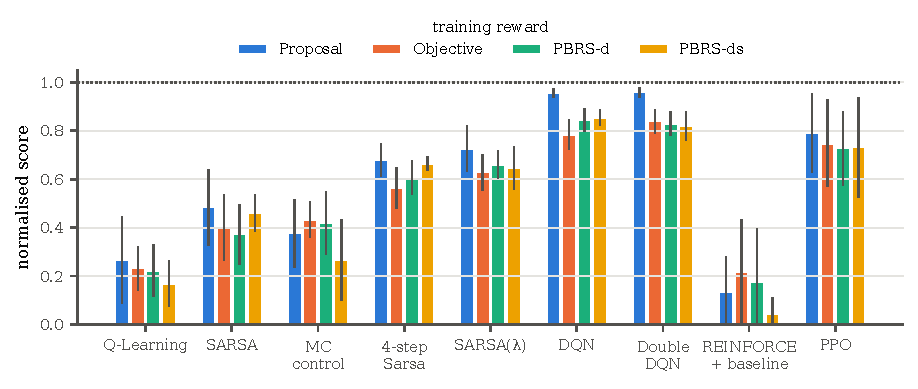
\includegraphics[width=\textwidth]{reward_effect}
\caption{Final normalised score of every learner under each training reward (mean and 95\% CI over 10 layouts). The dotted line is the best achievable behaviour.}
\label{fig:reward}
\end{figure*}

\begin{figure*}[t]
\centering
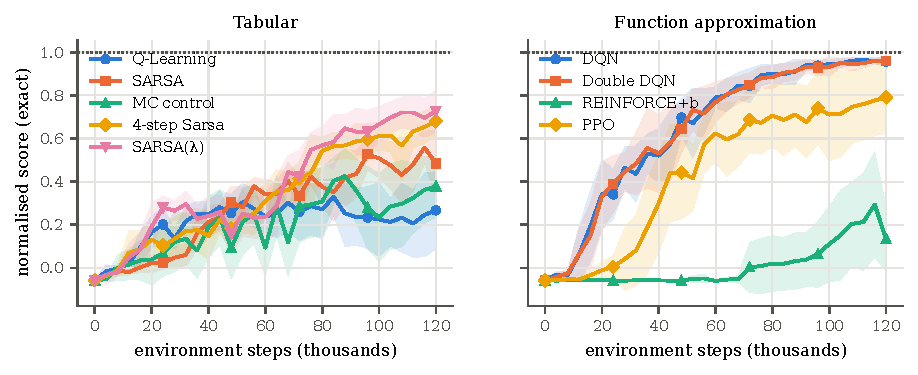
\includegraphics[width=\textwidth]{curves_proposal}
\caption{Learning curves under the Proposal reward: the exact normalised score of the current greedy policy every 20 runs (mean and 95\% CI over 10 layouts).}
\label{fig:curves}
\end{figure*}

\subsection{Operational metrics}
Table~\ref{tab:metrics} translates the scores into the six measures named in the project proposal, each defined so that it can be computed exactly: cumulative objective reward, service level (task completion), travel (energy), mean stockout duration (response time, the number of empty shelf-steps per shelf that ran out), load factor (resource utilisation, units per restock as a share of capacity) and, in Fig.~\ref{fig:curves}, convergence speed. DQN keeps shelves stocked 82\% of the time against 84.5\% for the optimum, and refills an empty shelf after 6.4 steps on average against 6.3. PPO shows how a mean can mislead: it has the largest share of proactive restocks, yet its mean stockout lasts 41 steps, because on the layouts where it stalls an empty shelf stays empty for most of the run. The tabular learners leave shelves empty for 11--67 steps.

\begin{table}[t]
\centering
\caption{Expected metrics per 200-step run for learners trained on the Proposal reward, beside the optimal policy (means over 10 layouts). $J$: objective; SL: service level; travel: moves; stockout: mean stockout duration (steps); proact.: share of restocks made before the shelf ran out; load: units per restock / capacity; opt.: probability of an optimal action on states $\pi^\ast$ visits.}
\label{tab:metrics}
\setlength{\tabcolsep}{2pt}
\footnotesize
\begin{tabular}{@{}lcccccccc@{}}
\toprule
 & score & $J$ & SL & travel & stockout & proact. & load & opt.\\
\midrule
\inputrows{tables/metrics_proposal.tex}
\bottomrule
\end{tabular}
\end{table}

\subsection{Which reward trains best, and why}
\label{sec:which}
Section~\ref{sec:audit} showed that the Proposal reward is slightly wrong at the optimum. Here it is the best training signal for seven of the nine learners, significantly so for 4-step Sarsa, SARSA($\lambda$), DQN and Double DQN (Table~\ref{tab:scores}). To find out which part of it helps, the restock bonus and the closer bonus were each added to the objective on their own (Table~\ref{tab:terms}).

For DQN both terms help, by $+0.12$ and $+0.10$, and the reward containing both reaches 0.96, up from 0.78. Their potential-based counterparts (PBRS-ds and PBRS-d) recover roughly half of each gain while provably leaving the optimal policy unchanged. The price of the larger gain is visible in behaviour: DQN trained on the Proposal reward travels further than the optimal policy on nine of the ten layouts. On layout~2, DQN and PPO both make about 140 moves per run where the optimum makes 120, and they sit to the right of the exact frontier (Fig.~\ref{fig:frontier}). The learners take the same loop that costs an optimal agent 0.3\% in score, and in exchange they reach a far better policy within the budget. At this training budget the Proposal reward is therefore the better choice, and the exact audit says what it costs.

\begin{table}[t]
\centering
\caption{One proposal term at a time (final score, mean of 10 layouts). $^\ast$: paired $p<0.05$ against Objective.}
\label{tab:terms}
\setlength{\tabcolsep}{2.2pt}
\footnotesize
\begin{tabular}{@{}lcccccc@{}}
\toprule
learner & Obj. & +restock & +closer & Proposal & PBRS-d & PBRS-ds\\
\midrule
\inputrows{tables/terms.tex}
\bottomrule
\end{tabular}
\end{table}

\begin{figure*}[t]
\centering
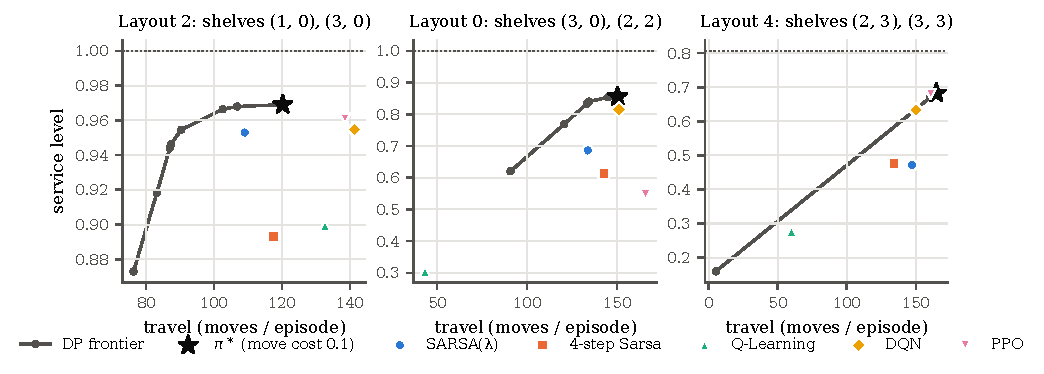
\includegraphics[width=\textwidth]{frontier_proposal}
\caption{Learned policies (Proposal reward) against the exact service--travel frontier of three layouts. The star is the optimum at the objective's travel price, and the dotted line is the travel-time bound. Points to the right of the frontier travel more than necessary for their service level.}
\label{fig:frontier}
\end{figure*}

\subsection{Why the tabular learners fall short}
\label{sec:why}
For the tabular learners, the reward explains less than it seems to. All five start from $Q_0=0$, and since the objective only ever charges, zero is above the optimal value of every state. Fig.~\ref{fig:diag} (left) measures how much of that optimism is left after training, as the gap between the learned values and $V^\ast$ on the states the optimal policy visits. One-step Q-Learning and SARSA still sit about 37--39 above $V^\ast$ after 120{,}000 steps: each update moves a value only a fraction $\alpha$ of the way toward a target that is itself too high. Eligibility traces and multi-step targets pass each correction back through many states at once and remove most of the gap (SARSA($\lambda$): $+7$). Monte Carlo, which never bootstraps, ends below $V^\ast$. Across layouts, the remaining optimism goes with a lower score.

Wiewiora's result~\cite{wiewiora2003} shows why shaping cannot remove this gap. For a tabular learner, adding $\gamma\Phi(s')-\Phi(s)$ to every reward is the same as starting from $Q_0(s,a)=\Phi(s)$. This was confirmed directly: with identical seeds, SARSA on PBRS-d and SARSA on the objective started from $\Phi$ visit the same states and keep tables that differ by exactly $\Phi(s)$ to $3\times10^{-14}$ for all 600 runs. PBRS-d therefore only lowers the starting values by twice the distance to the target shelf, at most 12, against an optimism of about 50, which is why it barely moves the tabular scores. The Proposal reward helps them for a related reason: its bonuses raise the true values, so the zero start is only about 20 above them instead of 55.

The causal test is to keep the objective and change only $Q_0$ (Table~\ref{tab:init}, Fig.~\ref{fig:init}). Starting at $-150$ triples Q-Learning's score (0.23 to 0.69) and lifts every TD learner significantly above its $Q_0=0$ result ($p\le0.001$). It also beats the Proposal reward started at zero, significantly for Q-Learning, SARSA and 4-step Sarsa ($p<0.01$) and narrowly for SARSA($\lambda$) (0.79 against 0.73, $p=0.10$). The effect has an inverted-U shape, with two failure modes that can be observed directly. Counting state--action visits during training on five layouts: with $Q_0=0$, the greedy action is the least-tried action in its state 9--16\% of the time, so the policy is pulled toward the actions it knows least about. With $Q_0=-300$ that never happens, but the greedy action has been tried thousands of times: the policy has locked onto early choices instead of comparing alternatives. The best constant, $-150$, lies close to the mean optimal value of the states an exploring agent visits ($-137$), between the largest ($-19$) and smallest ($-197$) optimal values. This is an observed coincidence, not a derived rule. Even at the best value, $Q_0=-150$, the trained values sit 67--82 \emph{below} $V^\ast$, so the greedy policy depends on how the leftover error is spread across the actions of a state more than on how accurate the values are. Monte Carlo is insensitive to $Q_0$, as expected for a method that never bootstraps.

\begin{figure*}[t]
\centering
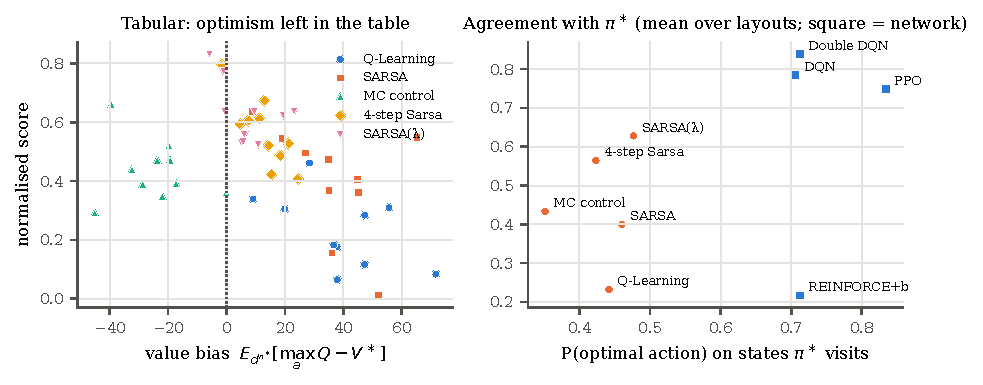
\includegraphics[width=\textwidth]{diagnostics_objective}
\caption{Inside the learned policies (Objective reward). Left: optimism left in each Q-table after training (one point per layout). Right: probability of choosing an optimal action on the states the optimal policy visits, against the score (one point per learner).}
\label{fig:diag}
\end{figure*}

\begin{figure}[t]
\centering
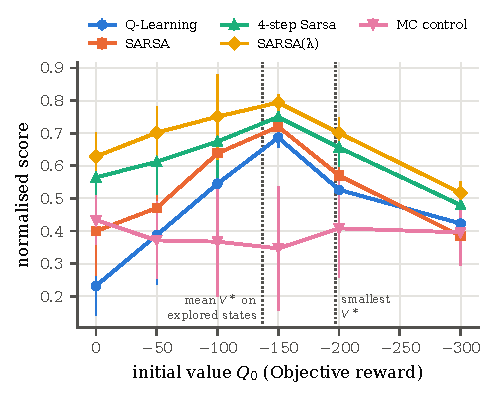
\includegraphics[width=\columnwidth]{init}
\caption{Tabular learners on the Objective reward with different initial values (mean and 95\% CI over 10 layouts). Dotted lines: mean optimal value of states an exploring agent visits, and the smallest optimal value.}
\label{fig:init}
\end{figure}

\begin{table}[t]
\centering
\caption{Final score on the Objective reward for initial values $Q_0$ (mean of 10 layouts; bold: best). For DQN, $Q_0$ is set through the output bias. Last column: Proposal reward with $Q_0=0$, for comparison.}
\label{tab:init}
\setlength{\tabcolsep}{2.4pt}
\footnotesize
\begin{tabular}{@{}lccccccc@{}}
\toprule
learner & 0 & $-50$ & $-100$ & $-150$ & $-200$ & $-300$ & Prop.\\
\midrule
\inputrows{tables/init.tex}
\bottomrule
\end{tabular}
\end{table}

None of this applies to DQN. Setting its output bias so that every initial value is $-150$ changes nothing for DQN (0.79 against 0.78, $p=0.80$) and makes Double DQN slightly worse (0.78 against 0.84, $p=0.02$). A network shares its parameters across states, so a few hundred updates rescale every output at once and no state keeps its initial value for long. For DQN, the gain from the Proposal reward is a genuine effect of its extra terms, as Table~\ref{tab:terms} showed.

\subsection{Greedy or stochastic policy-gradient agents}
\label{sec:stochastic}
REINFORCE and PPO learn a stochastic policy, and both forms were evaluated exactly. For REINFORCE the difference is large: its stochastic policy scores 0.45--0.49, while the argmax of the same policy scores 0.27--0.41 lower under every reward ($p\le0.012$). Reporting the argmax alone would understate what REINFORCE learned by more than half. For PPO the two forms agree on average (mean differences between $-0.04$ and $+0.03$), but on single layouts the gap reaches 0.62. Policy-gradient agents should therefore be evaluated with their stochastic policies.
